\documentclass[10pt]{extarticle}
\title{}
\author{Avinash Iyer}
\date{}
\usepackage[shortlabels]{enumitem}

%font setup
%
%\usepackage{newpxtext,eulerpx}

%paper setup
\usepackage{geometry}
\geometry{letterpaper, portrait, margin=1in}
\usepackage{fancyhdr}

%symbols
\usepackage{amsmath}
\usepackage{mathtools}
\usepackage{amsfonts}
\usepackage{hyperref}
\usepackage{gensymb}

\usepackage[T1]{fontenc}
\usepackage[utf8]{inputenc}

%chemistry stuff
%\usepackage[version=4]{mhchem}
%\usepackage{chemfig}

%plotting
\usepackage{pgfplots}
\usepackage{tikz}
\tikzset{middleweight/.style={pos = 0.5, fill=white}}
\tikzset{weight/.style={pos = 0.5, fill = white}}
\tikzset{lateweight/.style={pos = 0.75, fill = white}}
\tikzset{earlyweight/.style={pos = 0.25, fill=white}}
\usepackage{multirow,array}
%\usepackage{natbib}

%graphics stuff
\usepackage{graphicx}
\graphicspath{ {./images/} }

%code stuff
%when using minted, make sure to add the -shell-escape flag
%you can use lstlisting if you don't want to use minted
%\usepackage{minted}
%\usemintedstyle{pastie}
%\newminted[javacode]{java}{frame=lines,framesep=2mm,linenos=true,fontsize=\footnotesize,tabsize=3,autogobble,}
%\newminted[cppcode]{cpp}{frame=lines,framesep=2mm,linenos=true,fontsize=\footnotesize,tabsize=3,autogobble,}

%\usepackage{listings}
%\usepackage{color}
%\definecolor{dkgreen}{rgb}{0,0.6,0}
%\definecolor{gray}{rgb}{0.5,0.5,0.5}
%\definecolor{mauve}{rgb}{0.58,0,0.82}

%\lstset{frame=tb,
%	language=Java,
%	aboveskip=3mm,
%	belowskip=3mm,
%	showstringspaces=false,
%	columns=flexible,
%	basicstyle={\small\ttfamily},
%	numbers=none,
%	numberstyle=\tiny\color{gray},
%	keywordstyle=\color{blue},
%	commentstyle=\color{dkgreen},
%	stringstyle=\color{mauve},
%	breaklines=true,
%	breakatwhitespace=true,
%	tabsize=3
%}
% text + color boxes
\usepackage[most]{tcolorbox}
\tcbuselibrary{breakable}
\newtcolorbox{problem}[1]{colback = white, title = {#1}, breakable}
\newtcolorbox{solution}{colback = white, colframe = black!75!white, title = Solution, breakable}
%including PDFs
\usepackage{pdfpages}
\setlength{\parindent}{0pt}

\pagestyle{fancy}
\fancyhf{}
\rhead{Avinash Iyer}
\lhead{Econ 305: Class Notes}
\begin{document}
  \begin{problem}{Introduction to Game Theory}
    Game Theory analyzes the \textit{interaction} among a \textit{group} of \textit{rational} agents who \textit{behave strategically}.
    \begin{itemize}
      \item A group consists of at least two individuals who are free to make decisions.
      \item An interaction means that the decisions of at least one member of the group must affect at least one other member of the group.
      \item In strategic behavior, members of the group account for the interaction in their decision making process.
      \item Rational agents act in their best decisions based on their knowledge.
    \end{itemize}
    Keynes's Beauty Contest: Choose the face that is the most chosen in a newspaper contest.\\

    In many games, we are not asked to pick \textit{our} favorite, we are asked to pick \textit{everyone else's} favorite.
    \begin{problem}{Applications of Game Theory}
      \begin{itemize}
        \item Labor Economics (compensation interactions, promotions)
        \item Industrial Organization (pricing, entry, exit, etc.)
        \item Public Finance (public goods games)
        \item Political Economy (strategic voting)
        \item Trade (tariff wars)
        \item Biology (hunting and mating)
        \item Linguistics
      \end{itemize}
    \end{problem}
    It's important to remember that game theory is a subfield of \textit{mathematics}, not economics.
  \end{problem}
  \begin{problem}{Static Games of Complete Information}
    We will begin by covering \textit{static games of complete information}.
    \begin{itemize}
      \item Static: Play happens at once and payoffs are realized. Decisions are not necessarily made at the same time.
      \item Complete information: the following four are all common knowledge in the game
        \begin{enumerate}[(i)]
          \item all possible actions of the players
          \item all possible outcomes
          \item how each combination of actions of all players affects which outcome will materialize
          \item the preferences of each and every player over outcomes
        \end{enumerate}
      \item An event, $E$, is common knowledge if everyone knows $E$, everyone knows everyone knows $E$, \textit{ad infinitum}.
    \end{itemize}
    \begin{problem}{The Prisoner's Dilemma}
      \begin{itemize}
        \item Two suspects are interrogated in separate rooms.
        \item There is enough evidence to convict each of them for a minor offense, but not enough to convict either of a major crime unless one finks ($F$).
        \item If they each stay quiet ($Q$), they only get $1$ year in prison each.
        \item If only one finks, they are free, and the other gets $4$ years in prison.
        \item If they both fink, they each will spend $3$ years in prison.
      \end{itemize}
      We will try to write The Prisoner's Dilemma as a game. First, we can see this in a payoff matrix.
      \begin{center}
        \renewcommand{\arraystretch}{1.25}
        \begin{tabular}{cc|c|c|}
          & \multicolumn{1}{c}{} & \multicolumn{2}{c}{Player $Y$}\\
          & \multicolumn{1}{c}{} & \multicolumn{1}{c}{$Q$}  & \multicolumn{1}{c}{$F$} \\\cline{3-4}
          \multirow{2}*{Player $X$}  & $Q$ & $(2,2)$ & $(0,3)$ \\\cline{3-4}
          & $F$ & $(3,0)$ & $(1,1)$ \\\cline{3-4}
        \end{tabular}
      \end{center}
    \end{problem}
    \begin{problem}{Normal-Form Game}
      The constituents of a \textit{normal-form game} $G$ consist of the following:
      \begin{itemize}
        \item A finite set of players: $N = \{1,2,\dots,n\}$. 
        \item For each player $i$, a set $S_i$ denotes the \textit{strategy space} of player $i$. We will let $S = S_1\times S_2 \times \cdots S_n$ denote the strategy space of the entire game (i.e., the entire set of strategies possible).
          \begin{itemize}
            \item Every element $s\in S$ is a \textit{strategy profile}, where $s = (s_1,s_2,\dots,s_n)$. 
            \item We denote the strategy choices of all players except player $i$ as $s_{-i} = (s_1,\dots,s_{i-1},s_{i+1},\dots,s_n)$.
          \end{itemize}
        \item A payoff function: $v_i: S\rightarrow \mathbb{R}$. The payoff function depends on the strategies of \textit{all players}.
      \end{itemize}
      \begin{problem}{Example}
        Let the following payoff matrix represent a game. Write the normal form.
        \begin{center}
          \renewcommand{\arraystretch}{1.25}
          \begin{tabular}{c|c|c|}
            \multicolumn{1}{c}{} & \multicolumn{1}{c}{$X$} & \multicolumn{1}{c}{$Y$} \\\cline{2-3}
            $A$ & $(5,1)$ & $(2,6)$ \\\cline{2-3}
            $B$ & $(0,9)$ & $(3,2)$ \\\cline{2-3}
            $C$ & $(4,4)$ & $(4,7)$ \\\cline{2-3}
          \end{tabular}
        \end{center}
        \begin{itemize}
          \item $n = 2$
          \item $S_1 = \{A,B,C\}$\\
            $S_2 = \{X,Y\}$
        \end{itemize}
      \end{problem}
    \end{problem}
    \begin{problem}{Strategic Dominance}
      Recall the prisoner's dilemma.
      \begin{center}
        \renewcommand{\arraystretch}{1.25}
        \begin{tabular}{cc|c|c|}
          & \multicolumn{1}{c}{} & \multicolumn{2}{c}{Player $Y$}\\
          & \multicolumn{1}{c}{} & \multicolumn{1}{c}{$Q$}  & \multicolumn{1}{c}{$F$} \\\cline{3-4}
          \multirow{2}*{Player $X$}  & $Q$ & $(2,2)$ & $(0,3)$ \\\cline{3-4}
          & $F$ & $(3,0)$ & $(1,1)$ \\\cline{3-4}
        \end{tabular}
      \end{center}
      Suppose you were player 1. If player 2 stays quiet, it is more optimal for you to fink than to stay quiet. Similarly, if player 2 finks, then it is more optimal for you to fink than to stay quiet.\\

      In a similar vein, for player 2, it is more optimal to fink in both cases. Therefore, the proper strategy is $(F,F)$.\\

      \begin{problem}{Dominated Strategy}
        A strategy $s_i'$ if \textit{strictly dominated} for $i$ if there is one other strategy $s_i\in S_i$ such that $v_i(s_i,s_{-i}) > v_i(s_i',s_{-i})$ for all $s_{-i} \in S_{-i}$.\\

        Essentially, a strategy is strictly dominated if there is another strategy that yields a strictly greater payoff regardless of the other strategies.\\

        A rational player will \textit{never} play a strictly dominated strategy.
      \end{problem}
      In the prisoner's dilemma, $Q$ is strictly dominated by $F$ in both cases. Oddly, this yields the worst outcome from a social perspective (i.e., it has the lowest aggregate welfare).
      \begin{center}
        \renewcommand{\arraystretch}{1.25}
        \begin{tabular}{c|c|c|c|}
          \multicolumn{1}{c}{} & \multicolumn{1}{c}{$L$} & \multicolumn{1}{c}{$M$} & \multicolumn{1}{c}{$R$}\\\cline{2-4}
          $T$ & 2,2 & 1,1 & 4,0 \\\cline{2-4}
          $B$ & 1,2 & 4,1 & 3,5 \\\cline{2-4}
        \end{tabular}
      \end{center}
      Through \textit{iterated elimination of strictly dominated strategies} (IESDS), we start by removing $M$ from the strategy profile of player $2$ as playing $L$ is strictly better. Then, Player $1$ realizes that player $2$ is rational, and thus does not play $B$ (as $B$ is strictly dominated by $T$ once $M$ is removed from the strategy space of player $2$). Finally, Player $2$ does not play $R$, as $R$ is strictly dominated by $L$ given that player $1$ will play $T$. Thus, we get our answer of $\mathbf{T,L}$.\\

      A game is \textit{dominance solvable} if it can be solved via iterated elimination of strictly dominated strategies. However, only a small number of games are not dominance solvable.
    \end{problem}
  \end{problem}
  \begin{problem}{Strategic Dominance and Normal-Form Activity}
  \begin{tcbraster}[raster columns = 1,colframe=black!75!white,colback=white]
    \tcbincludepdf{images/activity_1.pdf}
  \end{tcbraster}
  \end{problem}
  \begin{problem}{Nash Equilibrium: Definition}
    A strategy profile $s^{*}$ is a \textit{pure strategy Nash equilibrium} if and only if the following holds.
    \[
      v_i(s^{*}_i,s^{*}_{-i}) \geq v_i (s_i,s^{*}_{-i})
    \] 
    for all players $i$ and all strategies $s_i\in S_i$.\\

    Given what all other players are doing, no single player has an incentive to deviate to another action. This does not inform us about how to get to the Nash equilibrium, it just tells us that it is one.\\

    For example, the prisoner's dilemma has a pure strategy Nash equilibrium: $(F,F)$
    \begin{itemize}
      \item For any other strategy profile, there is a profitable deviation.
      \item Similarly, result corresponds to the outcome of IESDS.
    \end{itemize}
    \begin{center}
      \renewcommand{\arraystretch}{1.25}
      \begin{tabular}{c|c|c|c|}
        \multicolumn{1}{c}{} & \multicolumn{1}{c}{$L$} & \multicolumn{1}{c}{$M$} & \multicolumn{1}{c}{$R$}\\\cline{2-4}
        $T$ & 2,2 & 1,1 & 4,0 \\\cline{2-4}
        $B$ & 1,2 & 4,1 & 3,5 \\\cline{2-4}
      \end{tabular}
    \end{center}
    In the above game, the pure strategy Nash equilibrium is $(T,L)$. We can easily check that it is a Nash equilibrium, but in order to check that it is unique, we would need to look for deviations from the other strategy profiles. Or do we?
  \end{problem}
  \begin{problem}{IESDS and Nash Equilibrium}
    \begin{itemize}
      \item If $s^*$ is a pure strategy Nash equilibrium of $G$, $s^*$ survives IESDS.
      \item An action that is played in a Nash equilibrium is never eliminated in IESDS.
      \item If $G$ is dominance solvable, then $G$ has a unique Nash equilibrium:
      \begin{itemize}
        \item The previous proposition tells us that $G$ is dominance solvable $\Rightarrow$ there is at most one Nash equilibrium.
      \end{itemize}
    \end{itemize}
    The relationship between the strategy set, $S$, the set of strategies that survive IESDS, and the Nash equilibrium can be seen below:
    \begin{center}
      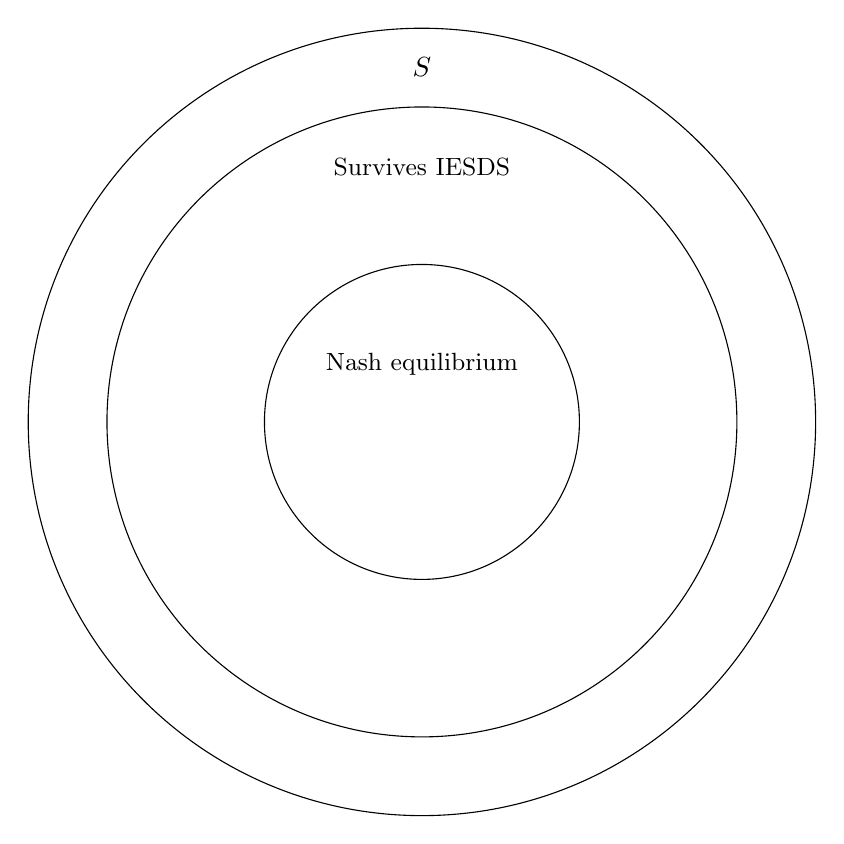
\begin{tikzpicture}
        \draw (0,0) circle (5cm);
        \draw (0,0) circle (4cm);
        \draw (0,0) circle (2cm);
        \node[anchor = north] at (0,4.75) {$S$};
        \node[anchor = south] at (0,3) {\small Survives IESDS};
        \node[anchor = north] at (0,1) {\small Nash equilibrium};
      \end{tikzpicture}
    \end{center}
  \end{problem}
  \begin{problem}{Voter Participation and Nash Equilibrium Activity}
    \begin{tcbraster}[raster columns = 1,colframe = black!75!white,colback=white]
      \tcbincludepdf{images/activity_2.pdf}
    \end{tcbraster}
  \end{problem}
  \begin{problem}{Bertrand Competition}
    \begin{description}
      \item[Assumptions] We have the following:
        \begin{description}
          \item[Players] Homogenous good produced by $n>1$ firms (i.e., oil, soybeans)
          \item[Cost] The cost of producing $q_i$ units to $c_i(q_i)$.
          \item[Demand] Total Market Demand is given by $D(p)$
          \item[Strategy Set] $S_i = \mathbb{R}^+$, where $p_i\in S_i$ denotes the price.
        \end{description}
      \item[Normal-Form Game] We have the following:
        \begin{description}
          \item[Players] $n=2$
          \item[Cost Function] $c_i(q_i) = cq_i$ for some $c\in \mathbb{R}^+$ and for $i=1,2$
          \item[Payoffs] $v_i(p_i,p_j) = \begin{cases}
              0, & p_i>p_j\\
              (p_i-c)(D(p_i)), & p_i<p_j\\
              \frac{1}{2}(p_i-c)(D(p_i)), & p_i=p_j
            \end{cases}$
        \end{description}
    \end{description}
  \end{problem}
  \begin{problem}{Bertrand Duopoly}
    \begin{tcbraster}[raster columns = 1,colframe = black!75!white,colback=white]
      \tcbincludepdf{images/activity_3.pdf}
    \end{tcbraster}
  \end{problem}
  \begin{problem}{Best Response Correspondence and finding Nash Equilibria}
    \begin{itemize}
      \item To find a Nash Equilibrium, it is helpful to determine which actions are best for a player given the actions of their opponents.
      \item A \textit{best response correspondence} is:
        \[
          BR_i(s_{-i}) = \{s_i\in S\mid v_i(s_i,s_{-i}) \geq v_i(s_i', s_{-i})~\forall s_i'\in S_i\}
        \] 
      \item Any strategy in $BR_i(s_{-i})$ is at least as good for player $i$ as every other strategy available to player $i$ when the other players' strategies are given by $s_{-i}$.
      \item We call it a correspondence, as oppposed to a function, since $BR_i(s_i)$ can be set-valued
    \end{itemize}
    A strategy profile $s^*$ is a Nash Equilibrium of $G$ if and only if every player's strategy is a best response to the other players' strategies:
    \[
      s^* \in BR_i(s^*_i)~\forall i
    \] 
    Essentially, every player is playing their best response given that everyone else is also playing their best response.\\

    There are two primary ways to find a Pure Strategy Nash Equilibrium:
    \begin{itemize}
      \item Refining educated guesses (e.g., Bertrand competition), necessary when best responses are set-valued
      \item Intersection of best responses (e.g., Payoff Matrix, Cournot competition)
    \end{itemize}
  \end{problem}
  \begin{problem}{Calculus and Best Response}
    In many cases, $BR_i(s_{-i})$ is a solution to the following problem:
    \[
      \max_{s_i}v_i(s_i,s_{-i})
    \] 
    Essentially, we have to solve an optimization problem: find the value of $s_i$ such that $v_i(s_i,s_{-i})$ is maximized.\\

    Consider the following payoff function:
    \[
      v_1(x_1,x_2) = 3x_1x_2 - x_1^2
    \] 
    We must use partial derivatives (as we're holding the strategy of $x_2$ constant in order to find the best response):
    \begin{align*}
      0 &= \frac{\partial v_1}{\partial x_1}\\
        &= 3x_2 - 2x_1\\
      x_1 &= \frac{3x_2}{2}
    \end{align*}
    Therefore, $BR_1(x_2) = x_1 = \frac{3x_2}{2}$.\\

    In order to find the Nash Equilibrium, we have to find the best response function for every player and take the intersections of all the best response functions.
  \end{problem}
  \begin{problem}{Cournot Competition}
    \begin{itemize}
      \item $n$ firms.
      \item Selling a homogenous identical good.
      \item \textit{Quantity} Competition: $S_i = \mathbb{R}^+$
      \item Payoff function:
        \[
          v_i(q_i,q_{-i}) = q_i P\left(\sum_{j = 1}^{n} q_j\right) - c(q_i)
        \] 
        What makes Cournot competition a game is that the payoff depends on the strategies of other players.
    \end{itemize}
  \end{problem}
  \begin{problem}{Cournot Duopoly: Example}
    \begin{itemize}
      \item $n=2$, $c(q_i) = 10q_i~\forall i$
      \item $P(Q) = \begin{cases}100-Q,&Q\leq 100\\0,&Q>100\end{cases}$
    \end{itemize}
    Three steps to find Nash Equilibrium:
    \begin{enumerate}[(i)]
      \item $BR_1(q_2)$
      \item $BR_2(q_1)$
      \item $(q_1^*,q_2^*)$ is a Nash Equilibrium where $q_1^* = BR_1(BR_2(q_1^*))$ (this follows from the definition of a Nash Equilibrium).
    \end{enumerate}
    \begin{align*}
      \max_{q_1} q_1(100-q_1-q_2)-10q_1 &= \max_{q_1} q_1(90-q_1-q_2)\\
      0 &= \frac{\partial v_1}{\partial q_1}\\
        &= 90-q_2-2q_1\\
      q_1 &= 45-\frac{1}{2}q_2
    \end{align*}
    \begin{align*}
      \max_{q_2} q_2(100-q_2-q_1)-10q_2 &= \max_{q_2}q_2(90-q_1-q_2)\\
      0&=\frac{\partial v_2}{q_2}\\
       &= 90-q_1-2q_2\\
      q_2 &= \frac{90-q_1}{2}
    \end{align*}
    \begin{description}
      \tiny
      \item[Note] In a symmetric game, every player's best response is identical with respect to every other player. You can only use this shortcut \textit{after} finding the best response.
    \end{description}
    \begin{align*}
      q_1^{*} &= BR_1(BR_2(q_1^*))\\
              &= \frac{90-\frac{90-q_1^*}{2}}{2}\\
              &= \frac{45}{2}+\frac{q_1^*}{4}\\
      q_1^* &= 30\\
      q_2^* &= BR(30)\\
            &= 30
    \end{align*}
    \begin{description}
      \tiny
      \item[Note] In a symmetric game, $q_1^* = q_2^*$, and similar for the $n$ player case.
    \end{description}
  \end{problem}
  \begin{problem}{Cournot Duopoly Variations}
    \begin{tcbraster}[raster columns = 1,colframe = black!75!white,colback=white]
      \tcbincludepdf{images/activity_4.pdf}
    \end{tcbraster}
  \end{problem}
\end{document}
